\pagebreak
\section{Model Component}

The application needs a model to represent recipes. The recipe data we receive from the server is of the \ac{json} format, the data is then parsed to our application model. The model component is shown in \autoref{fig:model}.

\begin{figure}[H]
\centering
\includegraphics[width=0.67\linewidth, page=2]{img/model.pdf}
\caption{Application model.}
\label{fig:model}
\end{figure}
We have two different representation of a recipe, \inline{Recipe} and \inline{IntermediateRecipe}. The \inline{IntermediateRecipe} is a small subset of a recipe which is used to display search results. When the user clicks one of the search results, then the rest of a \inline{Recipe} is downloaded from the server and displayed to the user.

A \inline{Recipe} consists of one or more instruction steps and one or more \linebreak\inline{IngredientGroups} which is a grouping of ingredients. An \inline{ExchangeableIngredient} consists of one or more \inline{IngredientQuantity} class which are interchangeable. 

\begin{figure}[H]
\centering
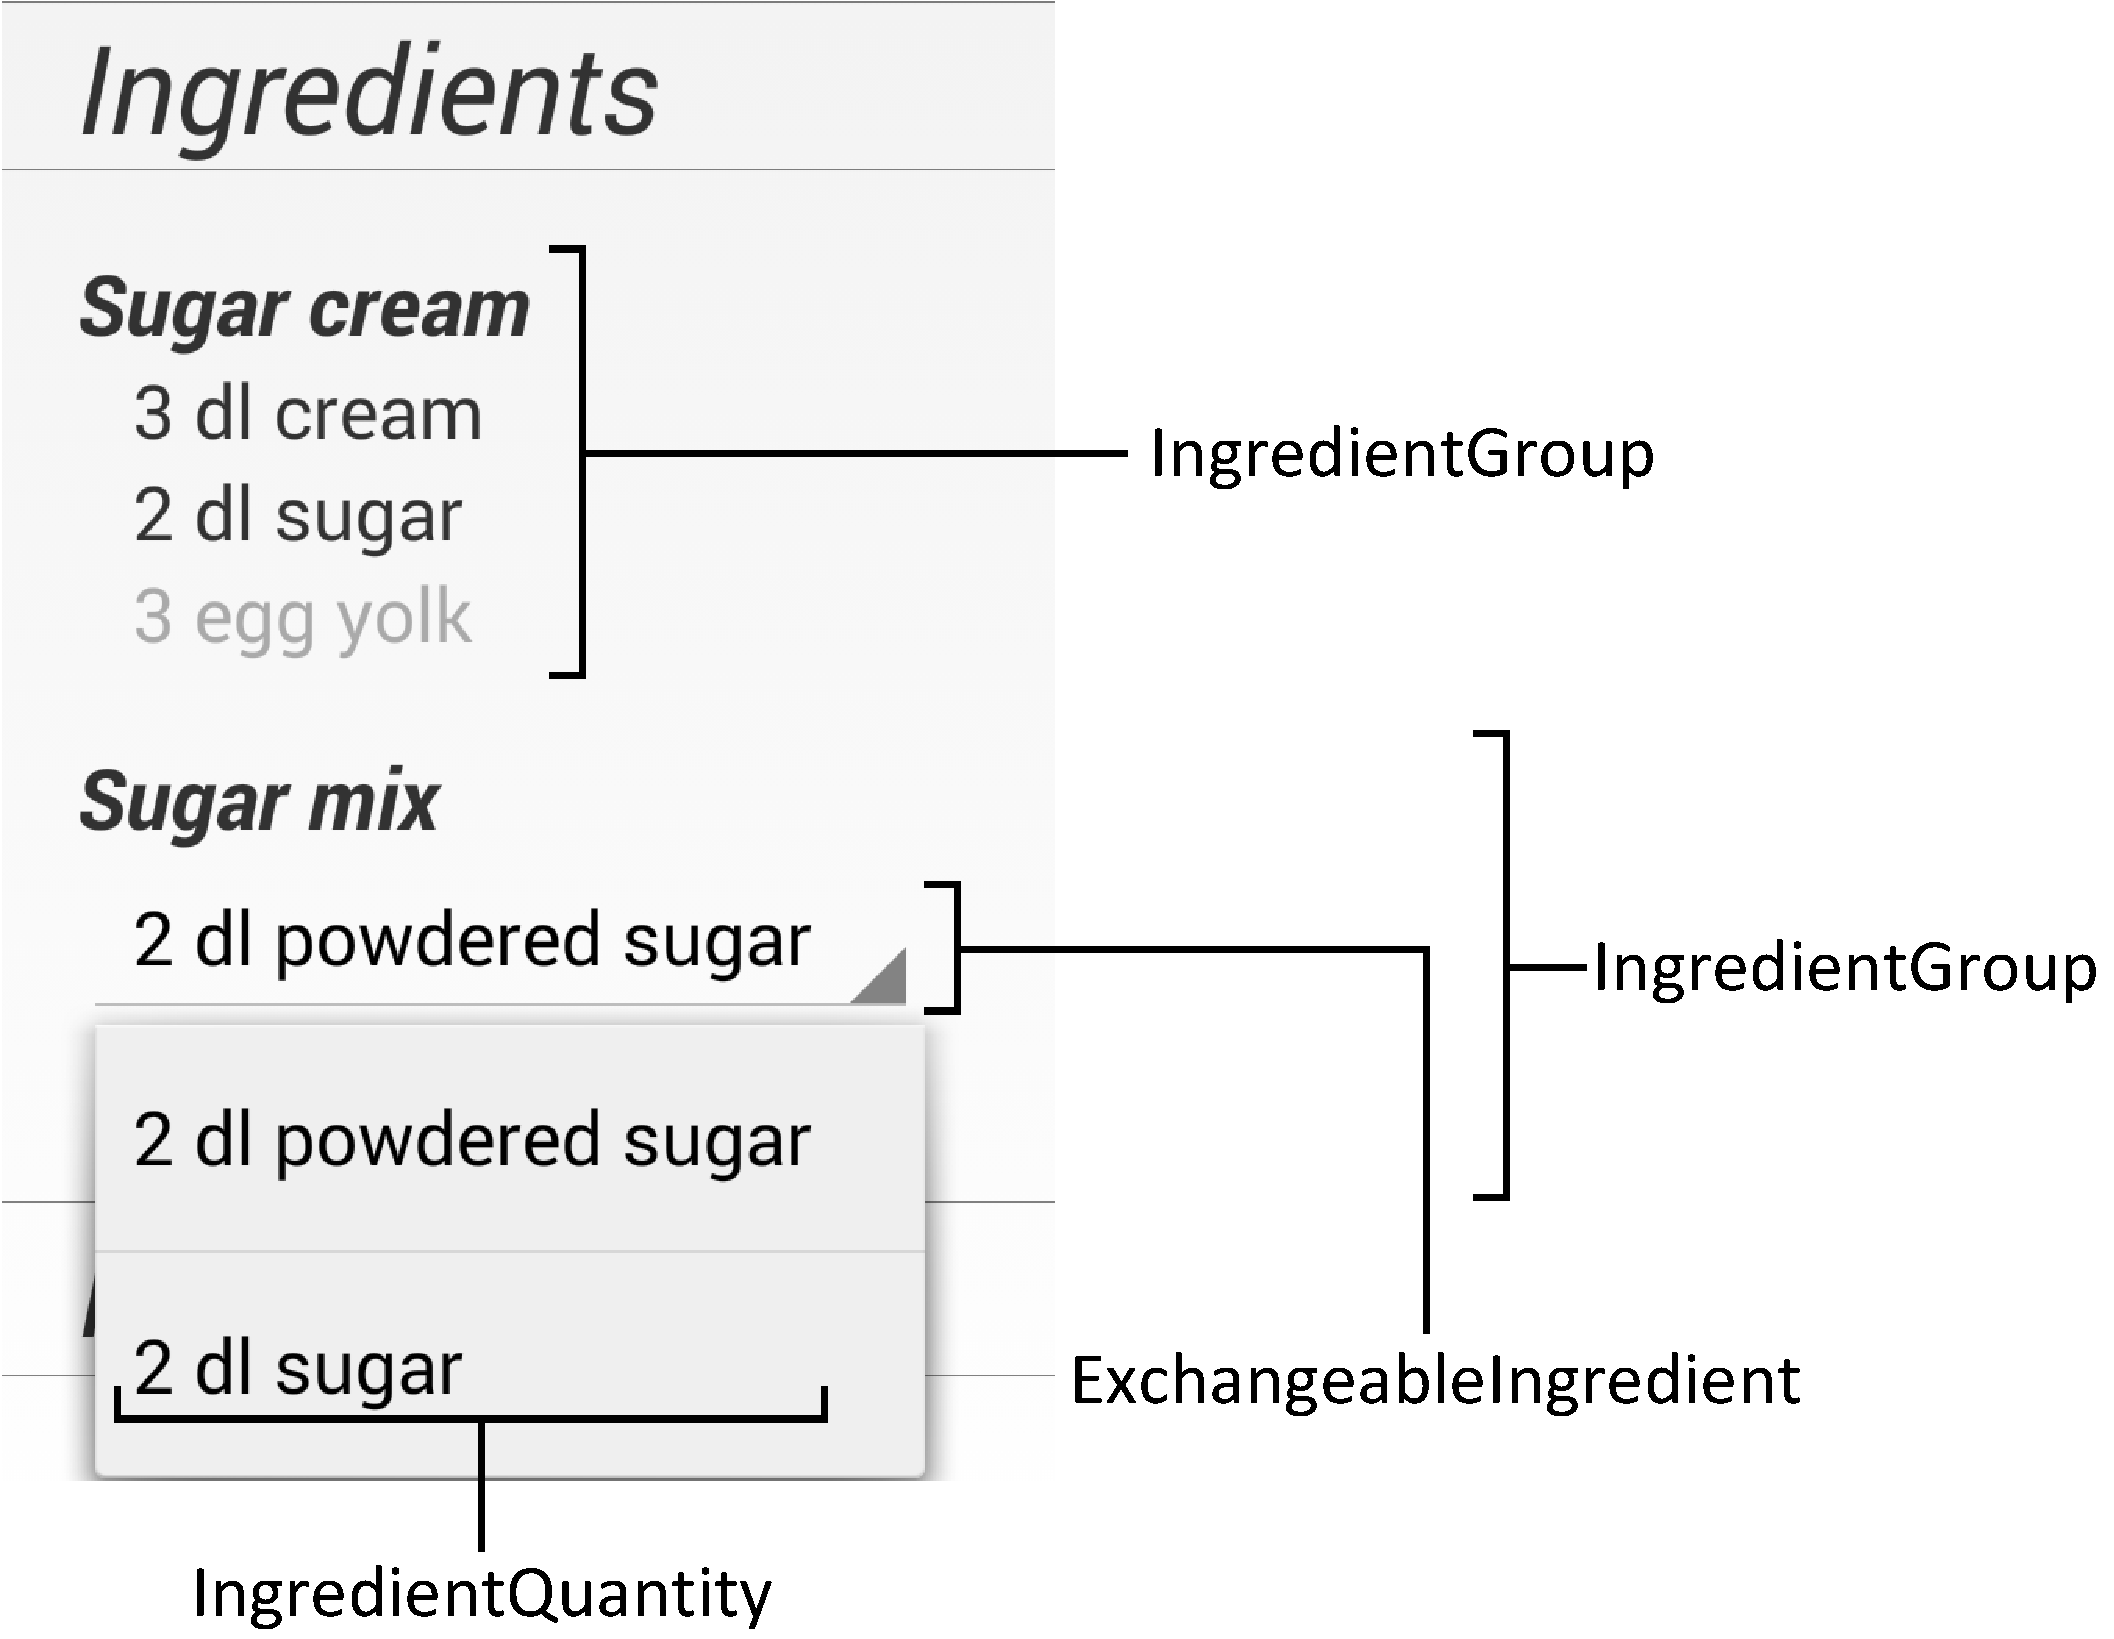
\includegraphics[width=0.6\linewidth]{img/ingredients.pdf}
\caption{Ingredient model.}
\label{fig:ingredients}
\end{figure}

The use of ingredients are easier understood by looking at \autoref{fig:ingredients}. If an ingredient can be exchanged by another ingredient, then it can be clicked which will reveal the different ingredients that can be used. It can be seen that \textit{2 dl powdered sugar} is exchangeable with \textit{2 dl sugar}.

The reason why the attributes from \inline{Unit} is not modelled inside \linebreak\inline{IngredientQuantity} is because the model resembles our relational database as much as possible. The \inline{Ingredient} class could also have been modelled inside \inline{IngredientQuantity}, but \inline{Ingredient} is used when searching by ingredients.